Eine der grundlegendsten Bedingungen dieser Arbeit ist, dass BLE als Technologie zum Übertragen der Daten zwischen Smartphone und Mikrocontroller genutzt werden soll. Demnach stellt sich die Frage nach einem geeigneten Transport der Daten innerhalb der BLE"=Architektur.
\\\\
Es existieren mehrere Referenzmodelle für die Kommunikation innerhalb von Rechnernetzen. Geläufig sind das TCP/IP"=Referenzmodell (Transport Control Protocol / Internet Protocol), das OSI"=Referenzmodell (Open Systems Interconnection) und ein hybrides Referenzmodell aus diesen beiden. Alle drei legen sich auf unterschiedliche Anzahlen von Schichten fest, von denen sich einige gleichen oder ähneln und andere nicht. Die Eigenschaften der Transportschicht sind bei den drei Referenzmodellen identisch. Die zu übertragenden Daten der darüberliegenden Anwendungsschicht werden in Segmente aufgeteilt und von einem Endpunkt über die niedrigeren Schichten zum anderen Endpunkt gesendet. Auf Empfängerseite erhält die Transportentität diese Segmente, setzt sie wiederzusammen und übergibt sie der zugehörigen Anwendung, die mithilfe von Ports identifiziert wird. Demnach kann die Transportschicht eine verbindungslose oder verbindungsorientierte Datenübertragung unterstützen, wobei die verbindungsorientierte Übertragung Flusskontrolle, verlustfreie Übertragung und die korrekte Reihenfolge der Segmente unterstützen kann. \cite{Baun2019_36-40}
% QUELLE https://katalog.ub.tu-freiberg.de/Record/0-1666728691, https://link.springer.com/book/10.1007%2F978-3-658-26356-0, Computer Networks / Computernetze von Christian Baun, S. 39 Transportschicht
\\\\
Die BLE"=Architektur lässt sich entsprechend der Abb. \ref{fig: hyb referenzmodell ble} am besten dem hybriden Referenzmodell zuordnen, da dieses im Gegensatz zum OSI-Referenzmodell die Anwendungsschicht nicht in drei weitere Schichten unterteilt und abgesehen von dieser Differenz dem OSI-Referenzmodell gleicht.

\begin{figure}[H]
    \centering
    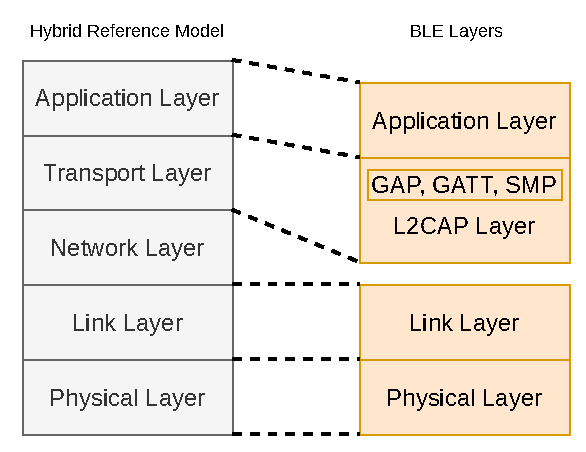
\includegraphics[width=0.55\textwidth]{graphics/hybr_referenzmodell_zu_ble.pdf}
    \caption[Zuordnung der BLE Layer zum hybriden Referenzmodell]{Zuordnung der BLE Layer zum hybriden Referenzmodell}
    \label{fig: hyb referenzmodell ble}
\end{figure}

Der Physical Layer bzgl. BLE stimmt mit dem Physical Layer des hybriden Referenzmodells überein, da hier die physikalische Bitübertragung definiert wird. Der Link Layer bzgl. BLE unterstützt wie der Link Layer des hybriden Referenzmodells den Zugriff auf das Übertragungsmedium mittels der Access Address und das Erkennen von fehlerhaft übertragenen Paketen (BLE) bzw. Frames (hybrides Referenzmodell) mittels einer Prüfsumme. Auch physische Adressen (zumindest die öffentliche Bluetooth"=Adresse) finden sich im Link Layer von BLE beim Advertising und Verbindungsaufbau wieder. Ein äquivalent zum Network Layer des hybriden Referenzmodells existiert nicht, da nur Punkt"=zu"=Punkt"=Verbindungen existieren, wodurch ein Routing der Pakete nicht nötig ist.
\\\\
L2CAP bzw. der L2CAP Layer kann als Äquivalent zum Transport Layer des hybriden Referenzmodells angesehen werden. Die Nutzdaten der Anwendungsschicht werden in Segmente aufgeteilt und über die niedrigeren Schichten an den L2CAP Layer des Empfängers übertragen. Über die L2CAP Channels und deren CIDs können diese Nutzdaten den Anwendungen zugeordnet werden. L2CAP ist in der Lage die Frames/PDUs verbindungsorientiert oder verbindungslos zu kommunizieren. Im LE Credit Based Flow Control Mode unterstützt BLE ab Bluetooth"=Version 4.2 Flusskontrolle. Eine verlustfreie Übertragung wird bereits im Link Layer bereitgestellt, da jedes Link"=Layer"=Paket vom Empfänger positiv (ACK) oder negativ (NAK) bestätigt wird. Wird ein Paket negativ bestätigt, wird es erneut gesendet.

Alle weiteren Protokolle wie GAP, SMP und GATT nutzen den Transport durch L2CAP. GAP dient dem Verbindungsaufbau und SMP bietet Sicherheitsfunktionen. Sie gehören im hybriden Referenzmodell dem "`oberen Teil"' des Transport Layers an.
\\\\
Ein wichtiger Schwerpunkt von BLE liegt in der Übertragung von Sensordaten \cite{BtDataTransfer}. Da GATT für die Übertragung von Sensordaten geeignet ist, tritt es häufig bei der Recherche nach der Funktionsweise und den Anwendungen von BLE auf. Jedoch basiert GATT seinem Namen entsprechend auf hierarchisch gegliederten Attributen, die unteranderem veränderbare Werte beinhalten. Ein Server erstellt solche Attribute und gibt diese über das Advertising oder erst über eine Verbindung zu einem Client bekannt. Der Client kann die Werte der Attribute mittels Anfragen lesen und schreiben. Der Server verfügt über die Attribute, wesewegen er diese zu jeder Zeit lesen und schreiben kann. Zudem kann der Server Attribute/Werte direkt an einen Client senden ohne eine vorherige Anfrage von diesem erhalten zu haben. 

Ein geeigneter Anwendungsfall wäre demnach ein Server, der über einen oder mehrere Sensoren verfügt, deren Ausgabewerte er zeitlich periodisch in seine vorher erstellten Attribute schreibt. Ein oder mehrere Clients können dann über die Attribute spezifische Sensordaten anfragen und empfangen.
\\\\
Daraus kann gefolgert werden, dass GATT im Gegensatz zum reinen L2CAP einen geringen Overhead benötigt und aufgrund seiner Architektur für diese Infrastruktur als Transportprotokoll eher ungeeignet ist. Trotzdem sei dem anzufügen, dass die meisten BLE"=Programmierschnittstellen den Zugang zu GATT ermöglichen.

Der Zugang zu L2CAP ist dagegen in einigen BLE"=Programmierschnittstellen nicht verfügbar. Ein Beispiel dafür sind die beiden gängigen Betriebssysteme Android und iOS. Android unterstützt BLE allgemein seit Android 4.3 \cite{AndroidAppLayerSec}, doch ermöglicht den Zugang zu L2CAP (also LE Connection"=Oriented Channels) erst ab Android 10 \cite{AndroidCoC}. iOS unterstützt BLE allgemein seit iOS 5.0 \cite{iOS_coreBluetooth} und ermöglicht den Zugang zu L2CAP erst ab iOS 11.0 \cite{iOS_CBL2CAPChannel}.
\\\\
Trotz des eingeschränkten Zugangs zu L2CAP in vielen Programmierschnittstellen, wird es als Transportprotokoll für diese Infrastruktur gewählt. Die Nutzung von GATT würde einen geringen Overhead erzeugen, da es ohnehin auf L2CAP basiert, und bis auf einen besseren Zugang keine weiteren Vorteile bieten.